\chapter{贪心法}


\section{Best Time to Buy and Sell Stock} %%%%%%%%%%%%%%%%%%%%%%%%%%%%%%
\label{sec:best-time-to-buy-and-sell-stock}


\subsubsection{描述}
Say you have an array for which the i-th element is the price of a given stock on day i.

If you were only permitted to complete at    most one transaction (ie, buy one and sell one share of the stock), design an algorithm to find the maximum profit.


\subsubsection{分析}
贪心法,分别找到价格最低和最高的一天,低进高出,注意最低的一天要在最高的一天之前。

把原始价格序列变成差分序列,本题也可以做是最大$m$子段和,$m=1$。

\subsubsection{代码}
\begin{Code}
class Solution {
public:
    int maxProfit(vector<int> &prices) {
        if (prices.size() < 2) return 0;
        int profit = 0;  // 差价,也就是利润
        int cur_min = prices[0]; // 当前最小

        for (int i = 1; i < prices.size(); i++) {
            profit = std::max(profit, prices[i] - cur_min);
            cur_min = std::min(cur_min, prices[i]);
        }
        return profit;
    }
};
\end{Code}


\subsubsection{相关题目}
\begindot
\item Best Time to Buy and Sell Stock II,见 \S \ref{sec:best-time-to-buy-and-sell-stock-ii}
\item Best Time to Buy and Sell Stock III,见 \S \ref{sec:best-time-to-buy-and-sell-stock-iii}
\myenddot


\section{Best Time to Buy and Sell Stock II} %%%%%%%%%%%%%%%%%%%%%%%%%%%%%%
\label{sec:best-time-to-buy-and-sell-stock-ii}


\subsubsection{描述}
Say you have an array for which the i-th element is the price of a given stock on day i.

Design an algorithm to find the maximum profit. You may complete as many transactions as you like (ie, buy one and sell one share of the stock multiple times). However, you may not engage in multiple transactions at the same time (ie, you must sell the stock before you buy again).


\subsubsection{分析}
贪心法,低进高出,把所有正的价格差价相加起来。

把原始价格序列变成差分序列,本题也可以做是最大$m$子段和,$m=$数组长度。

\subsubsection{代码}
\begin{Code}
class Solution {
public:
    int maxProfit(vector<int> &prices) {
        int sum = 0;
        for (int i = 1; i < prices.size(); i++) {
            int diff = prices[i] - prices[i - 1];
            if (diff > 0) sum += diff;
        }
        return sum;
    }
};
\end{Code}


\subsubsection{相关题目}
\begindot
\item Best Time to Buy and Sell Stock,见 \S \ref{sec:best-time-to-buy-and-sell-stock}
\item Best Time to Buy and Sell Stock III,见 \S \ref{sec:best-time-to-buy-and-sell-stock-iii}
\myenddot


\section{Longest Substring Without Repeating Characters} %%%%%%%%%%%%%%%%%%%%%%%%%%%%%%
\label{sec:longest-substring-without-repeating-characters}


\subsubsection{描述}
Given a string, find the length of the longest substring without repeating characters. For example, the longest substring without repeating letters for \code{"abcabcbb"} is \code{"abc"}, which the length is 3. For \code{"bbbbb"} the longest substring is \code{"b"}, with the length of 1.


\subsubsection{分析}
假设子串里含有重复字符,则父串一定含有重复字符,单个子问题就可以决定父问题,因此可以用贪心法。跟动规不同,动规里,单个子问题只能影响父问题,不足以决定父问题。

从左往右扫描,当遇到重复字母时,以上一个重复字母的\fn{index+1},作为新的搜索起始位置,直到最后一个字母,复杂度是$O(n)$。如图~\ref{fig:longest-substring-without-repeating-characters}所示。

\begin{center}
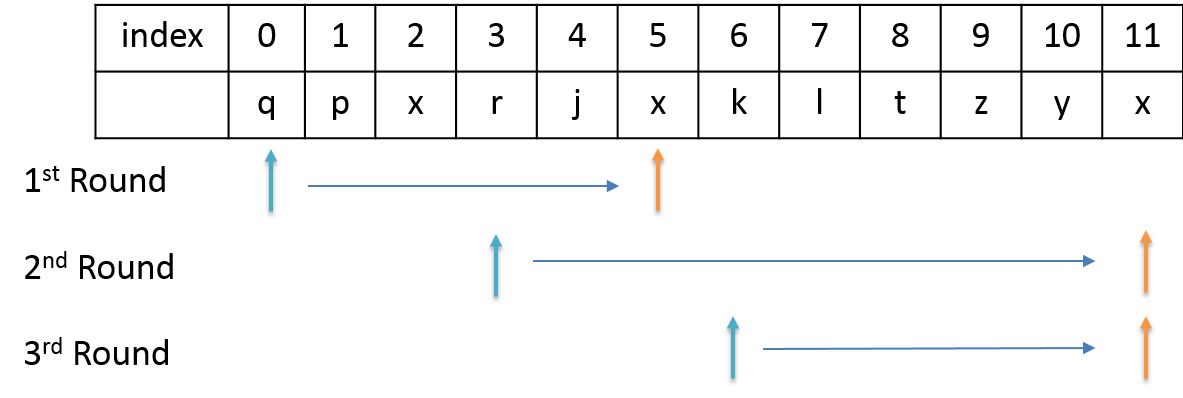
\includegraphics[width=300pt]{longest-substring-without-repeating-characters.png}\\
\figcaption{不含重复字符的最长子串}\label{fig:longest-substring-without-repeating-characters}
\end{center}


\subsubsection{代码}
\begin{Code}
// LeetCode, Longest Substring Without Repeating Characters
// 贪心法
class Solution {
public:
    int lengthOfLongestSubstring(string s) {
        const int ASCII_MAX = 26;
        int last[ASCII_MAX]; // 记录字符上次出现过的位置
        std::fill(last, last + ASCII_MAX, -1); // 0也是有效位置,因此初始化为-1
        int len = 0, max_len = 0;
        for (size_t i = 0; i < s.size(); i++, len++) {
            if (last[s[i] - 'a'] >= 0) {
                max_len = max(len, max_len);
                len = 0;
                i = last[s[i] - 'a'] + 1;
                std::fill(last, last + ASCII_MAX, -1);   // 重新开始
            }
            last[s[i] - 'a'] = i;
        }
        return max(len, max_len);  // 别忘了最后一次,例如"abcd"
    }
};
\end{Code}


\subsubsection{相关题目}
\begindot
\item 无
\myenddot
